% This file was converted to LaTeX by Writer2LaTeX ver. 1.4
% see http://writer2latex.sourceforge.net for more info
\documentclass{article}
\usepackage[latin1]{inputenc}
\usepackage[T3,T1]{fontenc}
\usepackage[english,swedish]{babel}
\usepackage[noenc]{tipa}
\usepackage{tipx}
\usepackage[geometry,weather,misc,clock]{ifsym}
\usepackage{pifont}
\usepackage{eurosym}
\usepackage{amsmath}
\usepackage{wasysym}
\usepackage{amssymb,amsfonts,textcomp}
\usepackage{array}
\usepackage{supertabular}
\usepackage{hhline}
\usepackage[pdftex]{graphicx}
\usepackage{float}
\usepackage{xr}

\makeatletter
\newcommand\arraybslash{\let\\\@arraycr}
\makeatother
\setlength\tabcolsep{1mm}
\renewcommand\arraystretch{1.3}
\newcounter{Table}
\renewcommand\theTable{\arabic{Table}}

\usepackage{lastpage}
\usepackage[hmargin=3cm,top=6cm,headheight=5cm,footskip=65pt]{geometry}

\usepackage{fancyhdr}
\fancyhf{}
\lhead{

\includegraphics[width=2cm]{figures/Arrowhead_logo}
}
\rhead{%
  \begin{tabular}{|p{8cm}|p{3cm}|}
\hline
    \small{Document title} & \small{Document type} \\
    Digital Twin & SoSD \\
    \small{Date} & \small{Version} \\
    \date{\today} & 1.0 \\
    \small{Author} & \small{Status} \\
    Jesper Frisk & Proposed \\
    \small{Contact} & \small{Page} \\
    jesfri-8@student.ltu.se & \thepage (\pageref{LastPage})\\ \hline
  \end{tabular}%
}

\lfoot{
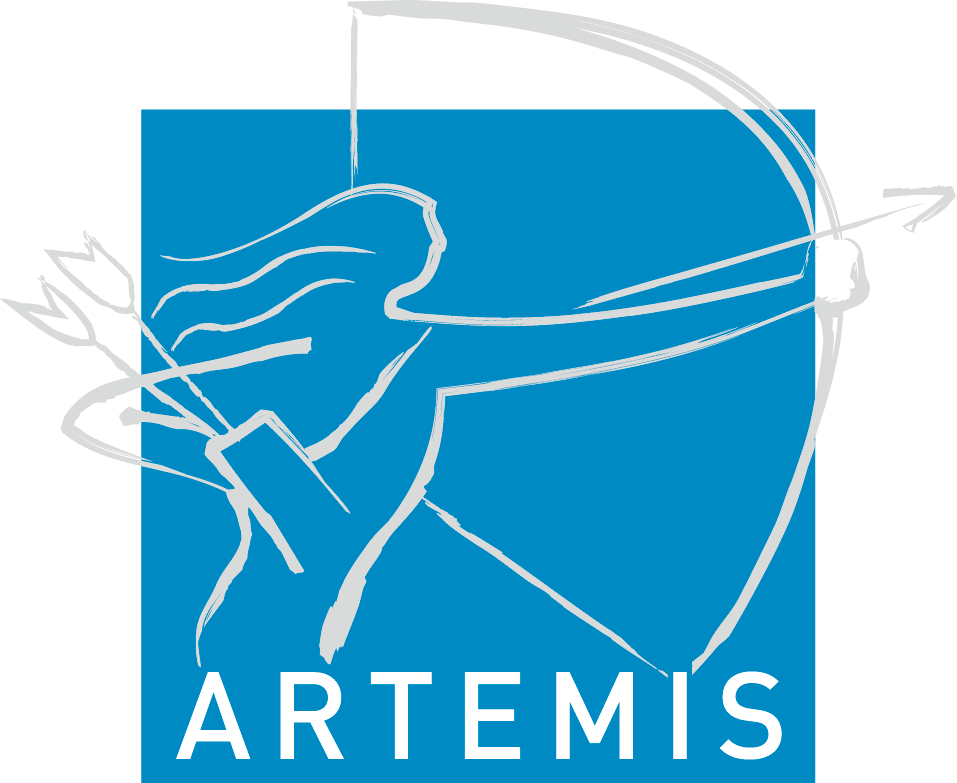
\includegraphics[width=2cm]{figures/Artemis_logo}
}
\rfoot{Contributed by the Arrowhead project, www.arrowhead.eu}

\renewcommand*{\headrulewidth}{0pt}
\pagestyle{fancy}




\title{System-of-Systems Description (SoSD) Digital Twin}
\begin{document}
\maketitle


\setcounter{tocdepth}{10}
\renewcommand\contentsname{}
\tableofcontents
\newpage

\section{System of Systems Overview}
Older robotics, micro controllers, PLCs and more can often have limitations to battery life availability and outdated communication protocols. This makes it difficult to have many different system that are based on modern communication protocols use their services. Instead a digital twin is created, this system connects to the robot, micro controller, PLC or other system via it's communication protocol and extends the functionalities of that system. In this document and accompanying documentation the system that is extended with a digital twin is referred to as a physical twin.

To create and host a digital twin a digital twin hub system is used. This system offers services to create and remove digital twins and it is responsible for the created digital twin. The digital twin hub hosts all necessary services for each digital twin, connects to the physical twin and saves necessary data for the digital twin. 

To demonstrate a created digital twin two different systems are used, a controller system that wants to send control commands to the physical twin, and a sensor system that wants to view sensor data from the physical twin. Furthermore a controller system is used in another cloud, to demonstrate inter cloud communication between the digital twin and other system that consumes it's services.

\begin{figure}[H]
    \centering
    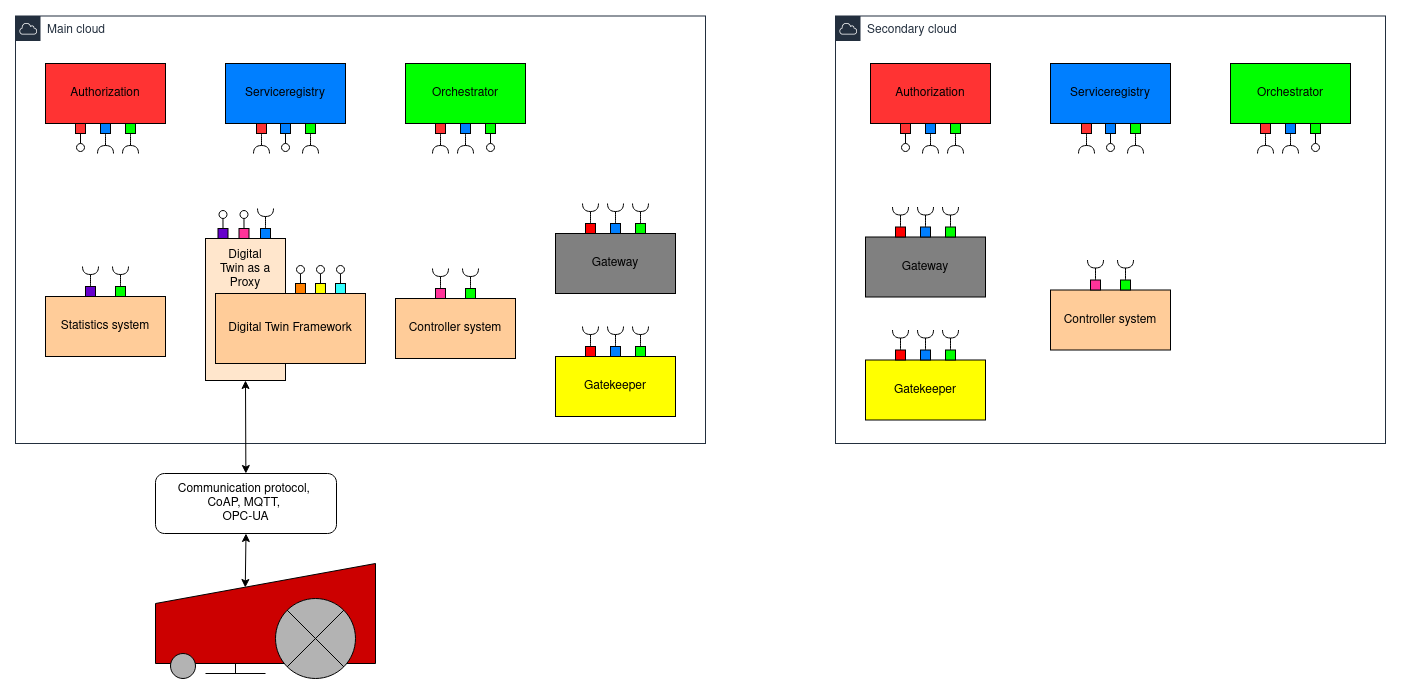
\includegraphics[width=\textwidth,height=\textheight,keepaspectratio]{figures/IoT-digital-twin-usecase.drawio.png}
    \caption{System architecture}
    \label{fig:architecture}
\end{figure}

\newpage

\section{Systems }

Table \stepcounter{Table}{\theTable} Pointers to the SysD documents

\begin{flushleft}
\tablefirsthead{}
\tablehead{}
\tabletail{}
\tablelasttail{}
\begin{supertabular}{|m{1.4531599in}|m{4.47956in}|}
\hline
System name &
Path\\\hline
Digital Twin Hub &
DigitalTwin/digital-twin-hub\_sysd.tex\\\hline
Digital Twin &
DigitalTwin/digital-twin\_sysd.tex\\\hline
Controller &
Controller/controller\_sysd.tex\\\hline
Sensor Retrieval &
SensorRetrieval/sensor-retrieval\_sysd.tex\\\hline
\end{supertabular}
\end{flushleft}

\newpage

\section{Use-cases}

Table \stepcounter{Table}{\theTable} Create Digital Twin Use-case description

\begin{flushleft}
\tablefirsthead{}
\tablehead{}
\tabletail{}
\tablelasttail{}
\begin{supertabular}{|m{6.01226in}|}
\hline
Create Digital Twin\\\hline
ID: 1 \\\hline
Brief description:

A system operator creates a new digital twin system.\\\hline

Primary actors:

Digital Twin Hub \\\hline
Secondary actors:

Physical Twin \\\hline
Preconditions:

The create process must be started by a system operator. \\\hline
Main flow:

1- The operator consumes the create-digital-twin service, and defines the connection to the physical twin and the services that the digital twin will extend.

2- The digital twin hub sets up the necessary communication to the physical twin as defined.

3- The digital twin hub sets up a rest api on a arbitrary and available port, and creates endpoints for all defined services that is extended from the physical twin. 

4- A new digital twin system is registered in the service registry, with all its accompanying services. 

5- Necessary data about the digital twin is saved in a local database.

\\\hline
Postconditions:

The digital twin hub is hosting a new digital twin, that can connect to the physical twin, and provides services that extends the physical twins functionalities, also all services created are registred in the service registry. \\\hline
Alternative flows:

Any possible alternative flows to the sequence presented in the Main flow section.\\\hline
\end{supertabular}
\end{flushleft}

\newpage

Table \stepcounter{Table}{\theTable} Remove Digital Twin Use-case description

\begin{flushleft}
\tablefirsthead{}
\tablehead{}
\tabletail{}
\tablelasttail{}
\begin{supertabular}{|m{6.01226in}|}
\hline
Remove Digital Twin\\\hline
ID: 2 \\\hline
Brief description:

A system operator removes a existing digital twin system.\\\hline

Primary actors:

Digital Twin Hub \\\hline
Secondary actors:

\\\hline
Preconditions:

The remove process must be started by a system operator. \\\hline
Main flow:

1- The operator consumes the remove-digital-twin service, and provides the address and port of the digital twin that is to be removed.

2- The digital twin hub shuts down the rest api of that digital twin.

3- The digital twin system and the accompanying services are unregistered from the service registry.

4- All saved data about the digital twin is removed from the digital twin hubs local database.

\\\hline
\end{supertabular}
\end{flushleft}

\newpage

Table \stepcounter{Table}{\theTable} Control a physical twin Use-case description

\begin{flushleft}
\tablefirsthead{}
\tablehead{}
\tabletail{}
\tablelasttail{}
\begin{supertabular}{|m{6.01226in}|}
\hline
Control a physical twin\\\hline
ID: 3 \\\hline
Brief description:

An application system consumes a service that is provided by a digital twin system, in order to control a physical twin. \\\hline

Primary actors:

Consuming application system, Digital Twin \\\hline
Secondary actors:

Physical Twin \\\hline
Preconditions:

The consuming application system orchestrates for a desired service. \\\hline
Main flow:

1- The application system consumes a control service provided by the digital twin, and forwards a control command.

2- The control command is forwarded to the physical twin.

3- The response of the control is returned to the application system.

\\\hline
Alternative flows:

If the physical twin cannot be reached by the digital twin system, an error is returned to the consuming application system.\\\hline
\end{supertabular}
\end{flushleft}

\begin{figure}[H]
    \centering
    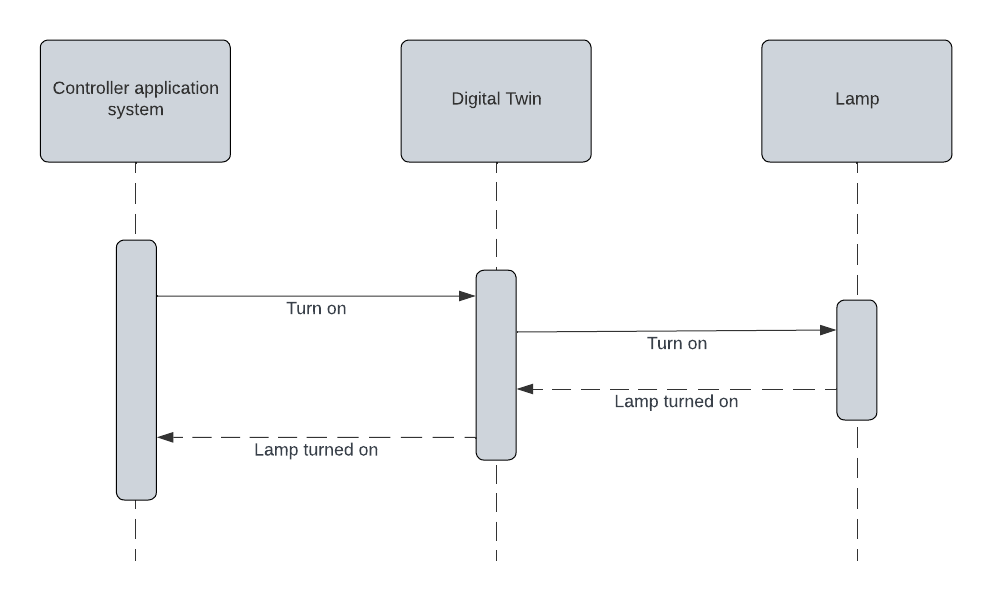
\includegraphics[width=\textwidth,height=\textheight,keepaspectratio]{./figures/Controller-Sequence.png}
    \caption{Sequence diagram of sending control commands, as an example the physical twin is in this case a lamp.}
    \label{fig:control-sequence}
\end{figure}

\newpage

Table \stepcounter{Table}{\theTable} Immediately view sensor data from physical twin Use-case description

\begin{flushleft}
\tablefirsthead{}
\tablehead{}
\tabletail{}
\tablelasttail{}
\begin{supertabular}{|m{6.01226in}|}
\hline
Immediately view sensor data from physical twin\\\hline
ID: 4 \\\hline
Brief description:

An application system consumes a service that is provided by a digital twin system, in order to view sensor data from a physical twin. \\\hline

Primary actors:

Consuming application system, Digital Twin \\\hline
Secondary actors:

Physical Twin \\\hline
Preconditions:

The consuming application system orchestrates for a desired service. \\\hline
Main flow:

1- The application system consumes a sensor service provided by the digital twin.

2- The sensor request is forwarded to the physical twin.

3- The sensor data is saved in the digital twin hubs database.

4- The sensor data is returned to the application system.

\\\hline
Alternative flows:

If the physical twin cannot be reached by the digital twin system, the latest data saved in the database is returned instead.\\\hline
\end{supertabular}
\end{flushleft}

\begin{figure}[H]
    \centering
    \includegraphics[width=\textwidth,height=\textheight,keepaspectratio]{./figures/Sensor-Sequence.png}
    \caption{Sequence diagram over immediate retrieval of sensor data, as an example the physical twin is in this case a temperature sensor.}
    \label{fig:sensor-sequence}
\end{figure}

\newpage

Table \stepcounter{Table}{\theTable} View sensor data from physical twin by interval retrieval Use-case description

\begin{flushleft}
\tablefirsthead{}
\tablehead{}
\tabletail{}
\tablelasttail{}
\begin{supertabular}{|m{6.01226in}|}
\hline
View sensor data from physical twin by interval retrieval\\\hline
ID: 5 \\\hline
Brief description:

An application system consumes a service that is provided by a digital twin system, in order to view sensor data from a physical twin. \\\hline

Primary actors:

Consuming application system, Digital Twin \\\hline
Secondary actors:

Physical Twin \\\hline
Preconditions:

The consuming application system orchestrates for a desired service. \\\hline
Main flow:

1- The digital twin asks the physical twin for the sensor data.

2- The sensor data is saved in the digital twin hubs database.

3- The application system consumes a sensor service provided by the digital twin.

4- The latest sensor data is retrieved from the database and returned to the application system.

\\\hline
\end{supertabular}
\end{flushleft}

\begin{figure}[H]
    \centering
    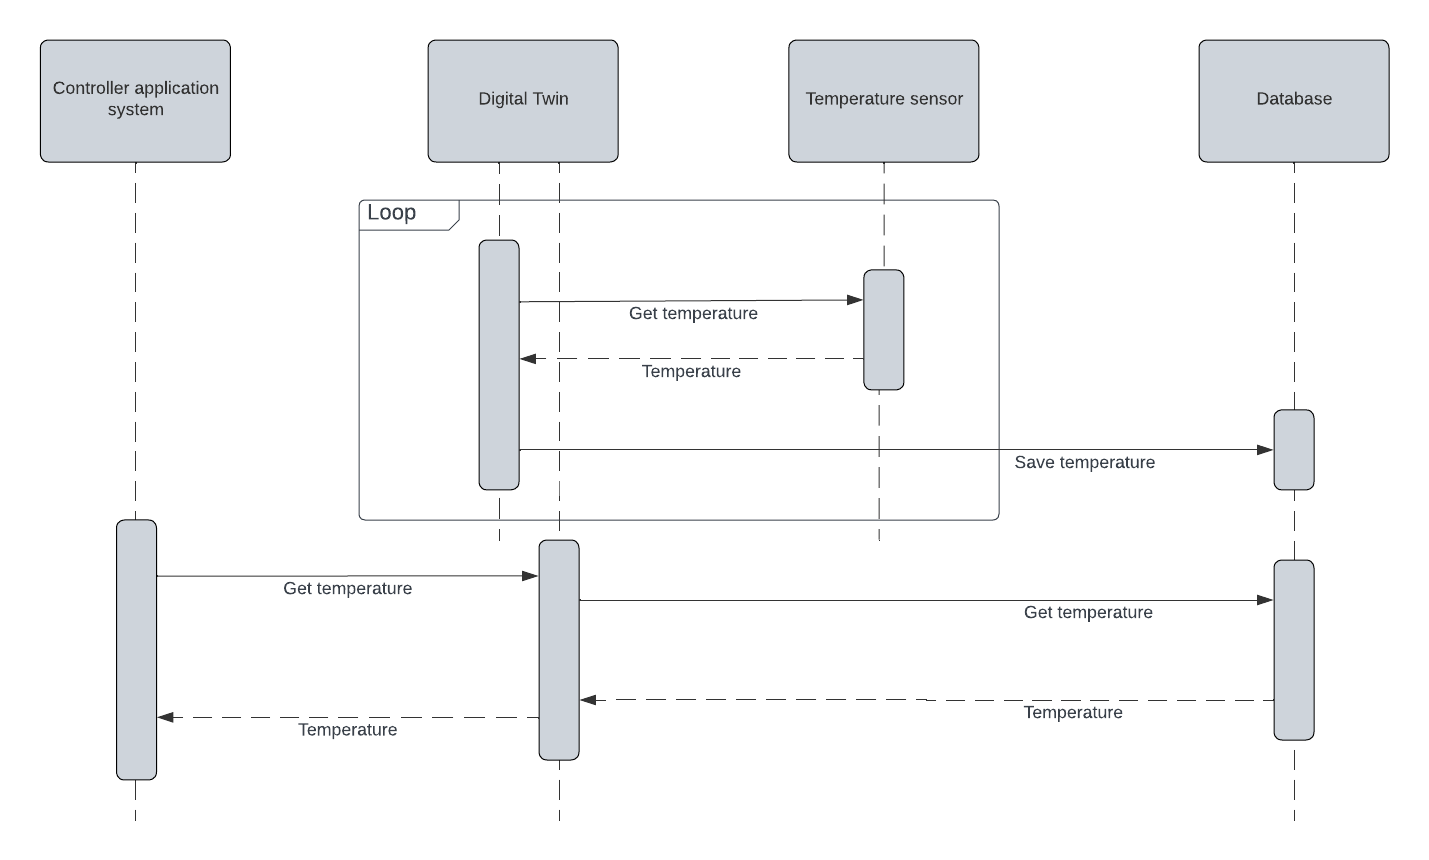
\includegraphics[width=\textwidth,height=\textheight,keepaspectratio]{./figures/Sensor-Interval-Sequence.png}
    \caption{Sequence diagram over interval retrieval of sensor data, as an example the physical twin is in this case a temperature sensor.}
    \label{fig:sensor-interval-sequence}
\end{figure}

\newpage

\section{Behaviour diagrams}
The diagrams proposed in this section are behaviour diagrams that provide a high level view of the SoS. The use of UML Activity diagrams, and BPMN or SysML Activity diagram is proposed.

The UML Activity diagrams are used to model a higher-level business process or processes.\ \ 

The BPMN diagrams provide a notation that is easily understandable by all business users. This includes the business analysts that create the initial drafts of the processes to the technical developers responsible for implementing the technology that will perform those processes.

The SysML diagrams support the specification, analysis, design, verification and validation systems that include hardware, software, data, personnel, procedures and facilities.

This section can also reports Sequence diagrams to specify how the involved systems interact with each other. The use of UML or SysML is proposed.

\section[Security ]{Security }

All systems use certificate security, and thus a valid certificate must be provided that follows the arrowhead certificate chain. To communicate with the Digital Twin hub a proper system operator certificate is needed.

\end{document}
